\skriptsection{Linear Discriminant Functions}{215}
  Assume, that the \em form \em of the discriminant functions are known instead of the
  distributions. The problem of finding a linear discriminant function can be formulated as a problem
  of \em minimizing a criterion function\em, e.g. \em the sample risk \em or \em training error\em.
  But a small training error doesn't guarantee a small \em test error\em.
  

  \skriptsubsection{Linear Discriminant Functions and Decision Surfaces}{216}
    \skriptsubsubsection{Two-Category Case}{216}
      The same forms as in summary chapter \ref{sec:bayes_discriminant_function} on page 
      \pageref{sec:bayes_discriminant_function} are used here.
      $$g(\bm x) = \bm w ^T \bm x + w_0$$
      Decide $\omega_1$ when $g(\bm x) > 0$ and $\omega_2$ when $g(\bm x) < 0$. $g(\bm x) = 0$ is
      the decision surface, it is a hyperplane in the linear case and it is normal to the weights 
      $\bm w$.
      
    \skriptsubsubsection{Multicategory Case}{218}
    \begin{minipage}{10.5cm}
      The linear machine should not be built using $c$ two-class classifiers or $c(c-1)/2$ linear
      discriminants to avoid unwanted ambiguous regions. Using $c$ linear discriminant 
      functions and vote or the highest value avoids this situation:
      $$g_i(\bm x) = \bm w_i^T \bm x + w_{i0} = w_0 + \sum\limits_{i=1}^d w_i x_i 
      \qquad \text{ with } i=1,\ldots,c$$
      $\bm x$ is assigned to $\omega_i$ when $g_i(\bm x) > g_j(\bm x)$. This is
      called a linear machine.
    \end{minipage}
    \begin{minipage}{4cm}
    	 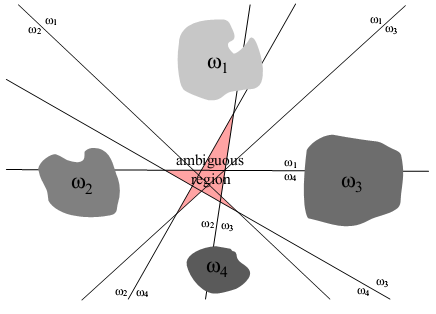
\includegraphics[width=4cm]{./images/ambiguousRegion.png}
    	 Ambiguous region because of split multicategory into multiple two-category problem
    \end{minipage}
    \hspace{1mm}
    \begin{minipage}{4cm}
    	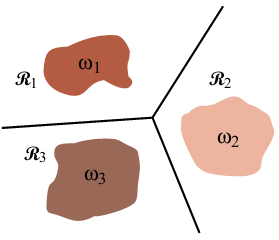
\includegraphics[width=4cm]{./images/regionWithVote.png}
    	Decision boundaries produced by voting.\\
    \end{minipage}
      
  
  \skriptsubsection{Generalized Linear Discriminant Functions}{219}
  \label{sec:generalized_linear_discriminant_function}
  \begin{minipage}{12cm}
    \subsubsection{Quadratic Discriminant Function}
    By multiplying features with itself, ``new'' features can be created and possibly improve the classification
    results. This results in the quadratic discriminant function\\
    $g(\bm x) = w_0 + \sum\limits_{i=1}^d w_i x_i + \sum\limits_{i=1}^d \sum\limits_{i=1}^d w_{ij} \underbrace{x_i x_j}_{\text{new feature}}$\\
    and can produce more complicated separating surfaces, because the problem will be mapped in a more dimensional space.
    The data itself uses not more dimensions. E.g. The data of an one dimension problem stays on one line.
  \end{minipage}
  \hspace{5mm}
  \begin{minipage}{6cm}
    	 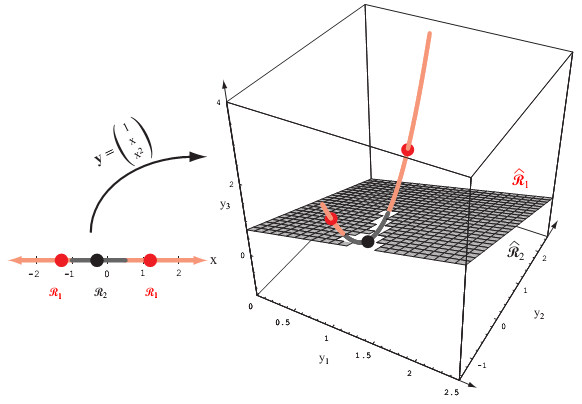
\includegraphics[width=6cm]{./images/map1DTo2D.png}
    	 Feature mapping from one dimension into 2D with $x^2$
  \end{minipage}
  
    \subsubsection{Generalized Linear Discriminant Functions}
    By continuing this approach, polynomial discriminant function or generalized linear discriminant 
    functions are evolving: 
    $$g(\bm x) = \sum\limits_{i=1}^{\hat d} a_i y_i(\bm x) = \bm a^T \bm y$$
    $\bm a$ is a 
    $\hat d$-dimensional weight vector and the $\hat d$ functions $y_i(\bm x)$ ($\varphi$-functions 
    or augmented features) are arbitrary functions of $\bm x$ and \textbf{don't have to be linear}.
    Therefore, the discriminant functions are linear in $\bm y$ but not in $\bm x$.\\
    The disadvantage is a high computational complexity with high dimensions and that much 
    \textbf{more trainings data} are needed to avoid overfitting.
     
    
    \subsubsection{Augmented Feature Vector}
    \begin{minipage}{12cm}
      To include the offset $w_0$ of the discriminant function $g(\bm x) = w_0 + w_1 x_1 + w_2 x_2 + \ldots + w_n x_d$ into the weight vector $\bm w$ 
      a one is added to the feature vector  $\bm y = [1, x_1, x_2, \ldots, x_n]^T = [1, \bm x]^T$.\\
      This vector is called \em augmented feature vector \em and the resulting weight vector $\bm a = [w_0, w_1, w_2, \ldots w_d]^T = [w_0, \bm w]^T$  \em augmented
      weight vector \em. \\
      The discriminant function can now be written as $g(x) = \bm a^T \bm y$.\\
      The decision boundary can now be interpreted as a hyperplane going through $[0,\ldots,0]$ and 
      all data lies on the level at $y_0=1$.\\
      Separation plane equation: $\bm a^T \cdot \bm y = 0$;  $\bm y = \begin{bmatrix}1 & x_1& x_2\end{bmatrix} \Rightarrow x_1=-\frac{a_0 + a_2\cdot x_2}{a_1}$
    \end{minipage}
    \hspace{5mm}
    \begin{minipage}{5cm}
    	 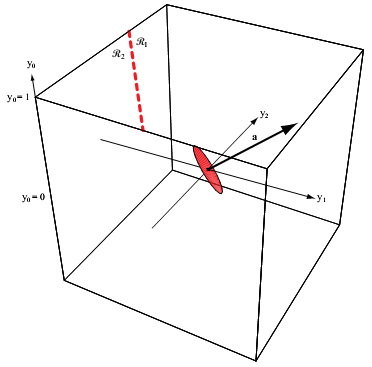
\includegraphics[width=5cm]{./images/augmentedVector.png}
   
    \end{minipage}
   
    
    
    
  \subsection{Two-Category Linearly Separable Case}
    If a linear weight vector exists that classifies all samples correctly, then the samples
    are said to be linearly separable.
    \begin{minipage}{11cm}
    
    \skriptsubsubsection{Normalisation / Margin}{223}
    In the separable case, the vector product of every training sample of class $\bm \omega_1$ with the solution
    vector $\bm a$ is positive, and with the class $\bm \omega_2$ is negative.\\
    For easier handling of the training data, one class is multiplied with $-1$. Now the vector product of the solution vector $\bm a$
     with \textbf{every} training sample will has to be positive $\bm a^T \bm y_i  > 0$\\\\
    The separating vector usually doesn't have one single solution but it can lie in a solution
    region. Furthermore, $\bm a$ should not lie on the boundary and therefore a margin $b$
    can be introduced.\\
        
    A normalized augmented feature for a 2-dimensional problem can then look like:
    $\bm y = \begin{bmatrix}
      1 & 1 & 2\\
      1 & 2 & 0\\
      -1 & -3 & -1\\
      -1 & -2 & -3
    \end{bmatrix}$.
    \end{minipage}
    \hspace{5mm}
    \begin{minipage}{7cm}
    	 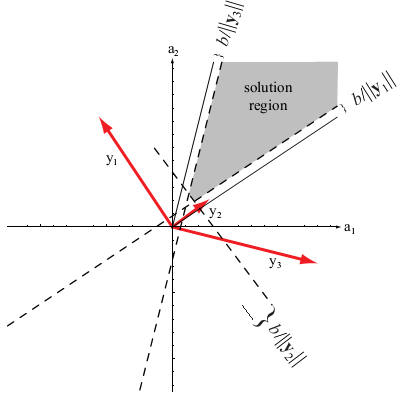
\includegraphics[width=7cm]{./images/solutionRegionWithMargin.png}
    	 Solution region of a ``normalized" vector with margin $b$
 	\end{minipage}
    
    \skriptsubsubsection{Basic Gradient Descent}{224}
      The basic approach to find a solution vector is the method of steepest descent. The aim is to
      minimize a defined criterion function $J_a$ and it is solved iteratively with every step calculating
      $$\bm a (1) \text{ arbitrary}$$
      $$\bm a (k+1) =  \bm a(k) - \eta(k) \nabla J(\bm a(k))$$
      with $\eta > 0$ being the step size or learning rate. When $\eta$ is too small, convergence is
      needlessly slow, with $\eta$ being large the correction can overshoot and even diverge.\\
      The \textbf{optimal step size} can be calculated with:
      $\eta(k)= \frac{\|\bm{\nabla J}\|^2}{\bm{\nabla J^T  H \nabla J}}$ where $\bm H$ is the Hessian matrix (see Newton's Algorithm).
      Calculating the Hessian matrix in every step is normally too expensive so that the optimal solution is used very seldom.

    \skriptsubsubsection{Newton's Algorithm}{226}
      The Newton method is not used widely due to the fact that a matrix has to be inverted on every
      step:
      $$\bm a(k+1) = \bm a(k) - \bm H^{-1} \bm \nabla \bm J \text{ with Hessian matrix } \bm H = \begin{bmatrix}
      \frac{\delta^2 f}{\delta x_1^2} & \ldots & \frac{\delta^2 f}{\delta x_1 \delta x_n}\\
      \vdots & \ddots & \vdots \\
      \frac{\delta^2 f}{\delta x_n \delta x_1} & \ldots & \frac{\delta^2 f}{\delta x_n^2}\\
      \end{bmatrix}$$
      This is a simplification of the optimum step size from the section above.
  
  \skriptsubsubsection{Minimizing the Perceptron Criterion Function}{227}
  \begin{minipage}{12cm}
    The problem is to construct a criterion function for solving the linear inequalities $\bm a^T \bm y > 0$. \\
    A criteria function which just counts the misclassified sample would be constant at the most position. Therefore the steepest descent would not work.
    
    A better idea is the \textbf{Perceptron Criterion Function}
    $\bm J_p(\bm a) = \sum\limits_{\bm y \in \mathcal{Y}_k} (-\bm a^T \bm y)$  with $\mathcal{Y}$ as the set
    of \textbf{misclassified samples} by the current weight vector $\bm a$.\\
    The gradient is $\bm {\nabla J}_p = \sum\limits_{\bm y\in \mathcal{Y}_k} -\bm y$
    and the update rule $\bm a(k+1) = \bm a(k) + \eta(k) \sum\limits_{\bm y\in \mathcal{Y}_k} \bm y$.
    
    
    \skriptsubsubsubsection{Batch Perceptron}{228}\\
    The \em batch perceptron algorithm \em yields in a solution for
    linearly separable problems. It sums up \em all \em misclassified samples and then performs a weight update (batch). 
    This has to be done until all of the samples will be classified correctly.
   	\end{minipage}
    \hspace{8mm} 
    \begin{minipage}{6cm}
    	 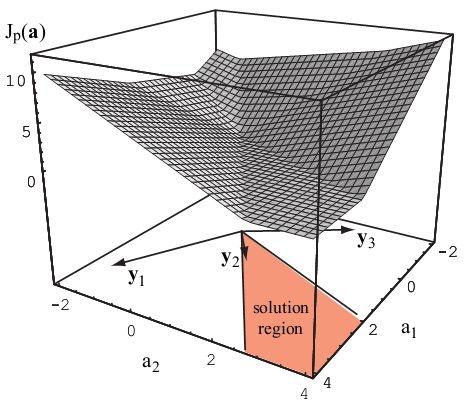
\includegraphics[width=6cm]{./images/perceptron.png}
    \end{minipage}
    
    
    \skriptsubsubsubsection{Fixed-Increment Single-Sample Perceptron}{230}\\
    The \em fixed-increment single-sample perceptron algorithm \em changes the weight vector
    with every (misclassified) sample and therefore saves many computations.
    
    \skriptsubsubsubsection{Variable-Increment Perceptron with Margin}{233}\\
    Additionally, the increment factor $\eta(k)$ can be variable. E.g. $\eta(k)=1/k$. For better 
    generalization, a margin $b$ can be added as shown in algorithm 5.  
    
    \skriptsubsubsection{Relaxation Procedures}{235}
    \begin{minipage}{12cm}
    The \em relaxation procedures \em use squares in the criterion function:\\
	$\bm J_q(\bm a) = \sum\limits_{\bm y \in \mathcal{Y}_k} (\bm a^T \bm y)^2$ with (again) $\mathcal{Y}$ as the set
    of \textbf{misclassified samples}.\\
  	Because the gradient is continuous, the criterion function $\bm J_q$ is smoother. The problem is that the algorithm is too smooth at the border and 
  	the algorithm can converge to the border or worse to $\bm a=0$. 
  	Another problem is that $\bm J_q$ is dominated by long training samples. A criterion function which solves both problems is:\\
  	$\bm J_r(\bm a) = \frac{1}{2} \sum\limits_{\bm y \in \mathcal{Y}_k} \frac{(\bm a^T \bm y - b)^2}{\|\bm y\|^2}$\\
  	where $b$ is a new margin and $\mathcal{Y}(\bm a)$ is the set of samples for which $\bm a^T \bm y \leq b$. $J_r$ is never 
  	negative and only zero when the whole set has been classified correctly inside margin.
	   
    \end{minipage}
    \hspace{8mm}
    \begin{minipage}{6.4cm}
    	 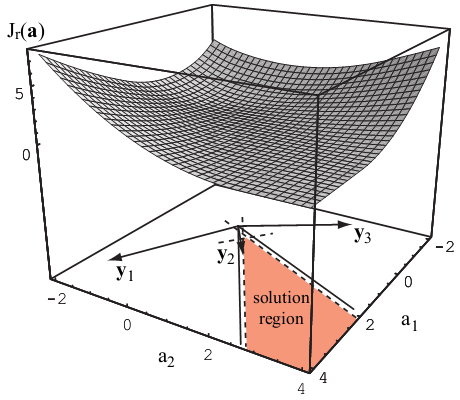
\includegraphics[width=6cm]{./images/relaxation.png}
    	 Criterion function of $\bm J_r(a)$ with margin $b$
    \end{minipage}
    
    \skriptsubsection{Nonseparable Behavior}{238}
    The algorithms up to now won't stop if the data is not separable. Moreover, we do not know if we get a ``good'' result if we stop after a long time.
    One way is to reduce the influence of the wrong classified sample with $\eta(k)=1/k$ so that the solution will end in a ``good'' area.
    
    \skriptsubsection{Minimum Squared-Error Procedures}{240}
    In comparison to the perceptron processes, here all samples are used. 
    The aim is $\bm a^T \bm y_i = b_i$ with $b_i$ to be specified. \\
    $\bm Y \bm a = \begin{bmatrix}
      y_{10} & y_{11} & \ldots & y_{1d}\\
      \vdots &\vdots & & \vdots\\
      \vdots &\vdots & & \vdots\\
      y_{n0} & y_{n1} & \ldots & y_{nd}\\
    \end{bmatrix}
    \begin{bmatrix}
    	a_0\\
    	\vdots\\
    	a_d
    \end{bmatrix} = 
    \begin{bmatrix}
    	b_0\\
    	\vdots\\
    	\vdots\\
    	b_n
    \end{bmatrix} = \bm b \qquad n \gg d$\\
    $b_i$ has to be a \textbf{positive} constant and is a kind of the margin. The criterion function 
    $\bm J_S(\bm a)=\|\bm Y \bm a - \bm b \|^2$ lead 
    us to the MSE solution $\bm a=\bm Y^\dagger \bm b$ of $\bm Y \bm a = \bm b$ 
    with the \em pseudoinverse \em $\bm Y^+= \bm Y^\dagger = (\bm Y^T \bm Y)^{-1} \bm Y^T$.
    Disadvantages of these algorithms are: High computational effort for computation of $\bm Y^\dagger$;
    possible singularities ($|\bm Y|$ close to zero); the separating vector is not necessarily found (see next figure);
    no clear abortion criterion (possibly: $|\eta(k) (\bm b - \bm a^T \bm y(k)) \bm y(k)| < \Theta$ with $\Theta$ being a threshold)\\
    
    $\bm Y$ is build as usual out of the augmented features vector of class 1 and the augmented features vector of class 2:\\
    $\bm Y = \begin{bmatrix}
    \bm 1_1 & \bm X_1 \\
    - \bm 1_2 & -\bm X_2  \\
    \end{bmatrix}$
    
    
    
    \begin{minipage}{12cm}
    \skriptsubsubsubsection{Algorithm: Widrow-Hoff / LMS Procedure}{245}\\
    To avoid large matrix multiplications the LMS procedure updates the weight vector with every sample. 
    In contrast to the previous algorithm the LMS use all samples.\\
    $$a(1) \text{ arbitrary}$$
  $$\bm a(k+1)=\bm a(k)+\eta(k)\left(\bm b-\bm a^T(k)\bm y(k)\right)\bm y(k)$$
    $\eta(k)$ has to decrease with $k$ to obtain convergence, e.g. $\eta(k)=n(1)/k$\\
    \end{minipage}
      \hspace{8mm}
      \begin{minipage}{6cm}
         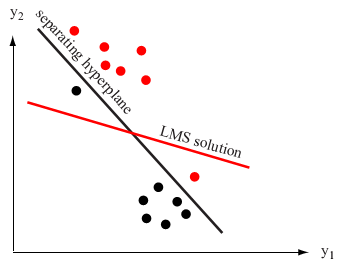
\includegraphics[width=6cm]{./images/LMS.png}
    \end{minipage}\\
    
    Different $\bm b$ lead to different interpretations / solutions:\\
    \begin{liste}
      \item 
        \skriptsubsubsubsection{Fisher's Linear Discriminant}{242}\\
        With $\bm b=\begin{bmatrix}
        \frac{n}{n_1} \cdot \bm 1_1\\
        \frac{n}{n_2} \cdot \bm 1_2
        \end{bmatrix}$ the pseudoinverse minimizes the ratio between the intra scatter $\bm S_i$ and the
        scatter within two classes $\bm S_W = \sum_i \bm S_i$.\\
      \item 
  \skriptsubsubsubsection{Asymptotic Approximation to an Optimal Discriminant}{243}\\
    With  $\bm b=\bm 1$ the pseudoinverse approximate to the Bayes discriminant function $g_0 = P(\omega_1 | \bm x) - P(\omega_2 | \bm x)$\\
    \end{liste}
    
     
    
 	
 	
 	\skriptsubsubsubsection{Stochastic Approximation Method}{247}\\
 	\todo{Danger: Might be wrong}
 	
 	The \em stochastic approximation method \em is almost the same as the LMS procedure. The different is, that the sample are token randomly. 
 	$$ \bm a(k+1)=a(k)+\eta(k)(\theta_k - \bm a^T(k)\bm y_k)\bm y_k$$
 	$\theta_k$ is $+1$ for $\omega_1$ and $-1$ for $\omega_2$. An important different is, that the vecotr $\bm y_k$ hasn't be ``normalized''. \\
 	$\eta(k)=1/k$ satisfy the convergence condition, but it converges often very slow. An optimal solution would be:
 	$$ \bm a(k+1)=a(k)+\bm R_{k+1}(\theta_k - \bm a^T(k)\bm y_k)\bm y_k$$
 	with $$\bm R_{k+1}^{-1}= \bm R_{k}^{-1} + \bm y_k \bm y_k^T$$ or
	$$\bm R_{k+1}= \bm R_{k} + \frac{\bm R_{k} \bm y_k(\bm R_{k} \bm y_k)^T}{1+\bm y_k^T \bm R_{k} \bm y_k}$$
 	$\bm R_{k}$ is the covariance matrix, which is updated every sample.
 	
 	
 	\skriptsubsection{Ho-Kashyap Procedures}{249}
 	The advantage of the \em Ho-Kashyap procedures \em is that the separating vector will be found in finite time, if the data is separable, or the 
 	solution will converge to the MSE solution in infinite time.
 	The idea is to adapt $\hat{\bm a}$ and $\hat{\bm b}$ in the MSE equation $\bm Y \hat{\bm a} = \hat{\bm b}$.
 	If the training samples are \textbf{lineary separable} a solution can be found so that 
 	\textbf{every component} $\hat{b_i}> 0$. Finally, $\bm e(k) = 0$ for a real solution or 
 	all $\bm e(k) \leq 0$ (all components not positive) when the samples are not linearly separable.\\
 	
 	\subsubsubsection{Descent Procedure}\\
 	The criterion function is the same as in LMS: $\bm J_S(\bm a)=\|\bm Y \bm a - \bm b \|^2$. But instead of updating only $\bm a$ vector $\bm b$
  is also updated:
 	$$ \bm b(k+1)=\bm b(k)- \eta(k) \frac{1}{2} \left(\bm{\nabla_b J}_s - |\bm{\nabla_b J}_s|\right) \qquad 
 	0 <\eta < 2/\lambda_{max} \; (\lambda \text{ are the eigenvalues of } \bm Y^T \bm Y)$$
 	$|\bm{\nabla_b J}_s|$ states that every component is positive. 
 	Gradient of $\bm J$ by $b$: $\bm{\nabla_b J}_s = 2\bm Y^T(\underbrace{\bm{Y a - b}}_{=e})$
 	
 	The only problem is, that the procedure only stops if the data are linear separable and convergence 
 	is only achieved in \textbf{finite} steps. There is no boundary of steps and hence, \textbf{when should be stopped?}\\
 	 
 	 
 	\skriptsubsubsubsection{Modified Ho-Kashyap}{254}
 	  The modified Ho-Kashyap uses the property that $\bm Y^\dagger \bm e(k) = 0$ and brings the advantage
 	  that the expensive pseudoinverse $\bm Y^\dagger$ has to be calculated only once at the start. It
 	  modifies the update rules compared to the general Ho-Kashyap and is always to be preferred.
 	  
 	  \begin{tabular}{lll}
 	    Init 
 	      &$\bm b(1) > 0$ (arbitrary) 
 	      &$\bm a(1) = \bm Y^\dagger \bm b(1)$\\
 	    Update 
 	      &$\bm b(k+1) = \bm b(k) + \eta (\underbrace{\bm e(k) + |\bm e(k)|}_{2e^+})$ 
 	      &$\bm a(k+1) = \bm a(k) + \eta \bm Y^\dagger |\bm e(k)|$
    \end{tabular}
 	
 	\skriptsubsubsubsection{Related Procedures}{254}
 	  This approach avoids the computation of $\bm Y^\dagger$ by introducing a matrix $\bm R$. 
 	  
    \begin{tabular}{lll}
      Init 
        &$\bm b(1) > 0$ (arbitrary) 
        &$\bm a(1)$ (arbitrary)\\
      Update 
        &$\bm b(k+1) = \bm b(k) + \eta (\bm e(k) + |\bm e(k)|)$ 
        &$\bm a(k+1) = \bm a(k) + \eta \bm R \bm Y^T |\bm e(k)|$
    \end{tabular}
 	  
 	  When $\bm R = \bm 1$ the step size becomes $\eta(k) = \frac{\|\bm Y^T |e(k|)\|^2}{\|\bm Y \bm Y^T |e(k)|\|^2}$.\\
 	  When $\bm R = \frac{1}{\eta} (\bm Y^T \bm Y)^{-1}$ this procedure becomes the original Ho-Kashyap.
 	
 	
 	\skriptsubsection{Overview over Different Procedures}{260} 
 	
 	\skriptsubsection{Multicategory Generalization}{265}
 	To handle \em multicategory cases \em with the \textbf{Kesler's Construction} the dimension of 
 	the weight vector $\bm a$ has to be extended by factor $c$
 	 and $(c-1)c$ new training samples generated:
 	$$ \bm{ \hat{a} }=\begin{bmatrix}
 	\bm a_1\\
 	\bm a_2\\
 	\vdots\\
 	\bm a_c
 	\end{bmatrix} \quad \text{and} \quad \bm \eta_{12}=\begin{bmatrix}
 	\bm y\\
 	-\bm y\\
 	\bm 0\\
 	\vdots\\
 	\bm 0
 	\end{bmatrix}; \quad \bm \eta_{13}=\begin{bmatrix}
 	\bm y\\
 	\bm 0\\
 	- \bm y\\
 	\vdots\\
 	\bm 0
 	\end{bmatrix}, \quad \ldots,\quad \bm \eta_{1c}=\begin{bmatrix}
 	\bm y\\
 	\bm 0\\
 	\bm 0\\
 	\vdots\\
 	-\bm y
 	\end{bmatrix}
 	$$
 	$c$ is the number of classes. Now the problem is again a two class problem. The solution solves the inequality:
 	$$\bm{\hat{a}}^T\bm \eta_{ji}>0$$
 	if the problem is linear separable. T
 	his idea is working for the most procedures except for the MSE or linear programming approaches (see \formelbuch{268})..
 	The fact that this needs many more samples is not practical but it allows us to convert many 
 	multi-category problems into two-category problems.
 	